\documentclass[a4paper,12pt]{article} 

%%% Работа с русским языком
\usepackage{cmap}                           % поиск в PDF
\usepackage{mathtext} 			 	       % русские буквы в формулах
\usepackage[T2A]{fontenc}               % кодировка
\usepackage[utf8]{inputenc}              % кодировка исходного текста
\usepackage[english,russian]{babel}  % локализация и переносы


\usepackage{wrapfig}


%Матеша
\usepackage{amsmath,amsfonts,amssymb,amsthm,mathtools} % AMS
\usepackage{icomma} % "Умная" запятая

%\mathtoolsset{showonlyrefs=true} % Показывать номера только у тех формул, на которые есть \eqref{} в тексте.

%% Шрифты
\usepackage{euscript}	 % Шрифт Евклид
\usepackage{mathrsfs} % Красивый матшрифт

%% Свои команды
\DeclareMathOperator{\sgn}{\mathop{sgn}}

%% Перенос знаков в формулах (по Львовскому)
\newcommand*{\hm}[1]{#1\nobreak\discretionary{}
	{\hbox{$\mathsurround=0pt #1$}}{}}



%%% Заголовок
\author
{
	\vspace*{15 cm}		
	Строчук Андрей Б01-103
}
\title{Лабораторная работа 2.3.1

Получение и измерение вакуума}
\date{\today}


\begin{document}
\maketitle

\newpage

\paragraph{Цель работы:}
1) измерение объемов форвакуумной и высоковакуумной частей установки;
2) определение скорости откачки системы в стационарном режиме, а также по ухудшению и улучшению вакуума.
\paragraph{В работе используются:} вакуумная установка с манометрами: масляным, термопарным и ионизационным.




В данной работе используются традиционные методы откачки механическим форвакуумным насосом до давления $10^{-2}$ торр и диффузионным масляным насосом до давления $10^{-5}$ торр, а также методы измерения вакуума в этом диапозоне. 


\subparagraph*{Экспериментальная установка.} 
 	Установка изготовлена из стекла,
 и состоит из форвакуумного баллона (ФБ), высоковакуумного диффузионного насоса (ВН), высоковакуумного баллона (ВБ), масляного (М) и ионизационного (И) манометров, термопарных манометров ($\text{М}_1$ и $\text{М}_2$), форвакуумного насоса (ФН) и соединительных кранов ($К_1, К_2,..., К_6$) (Рис. 1). Кроме того, в состав установки входят: вариатор (автотрансформатор с регулируемым выходным напряжением), или реостат и амперметр для регулирования тока нагревателя диффузионного насоса. \\
  \begin{figure}[h]
 	\centering
 	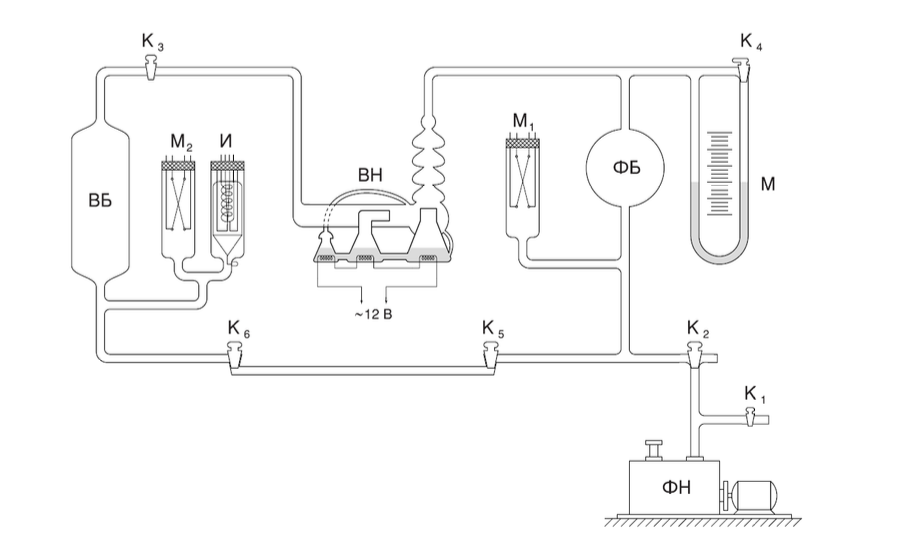
\includegraphics[width=0.7 \textheight]{1.jpg}
 	\caption{Схема установки}
 	\label{fig:Схема установки}
 \end{figure}

Кран $К_1$ используется для заполнения форвакуумного насоса и вакуумной установки атмосферным воздухом. Во время работы установки
он должен быть закрыт. Трёхходовой кран $К_2$ служит для соединения
форвакуумного насоса с установкой или атмосферой. Кран $К_3$ отделяет
высоковакуумную часть установки от форвакуумной. Кран $К_4$ соединяет между собой колена масляного манометра. Он должен быть открыт во все время работы установки и закрывается лишь при измерении
давления в форвакуумной части. Краны $К_5$ и $К_6$ стоят по концам капилляра и соединяют его с форвакуумной и высоковакуумной частями установки. 



\begin{figure}[t]
	\centering
	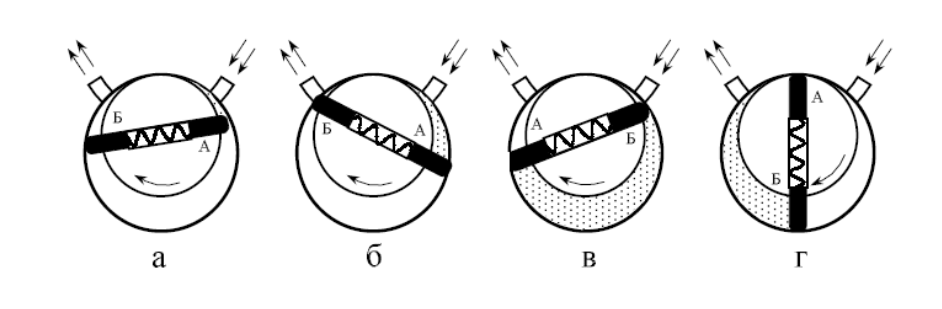
\includegraphics[width=0.9\linewidth]{2.jpg}
	\caption[]{Схема действия ротационного двухпластинчатого форвакуумного насоса}
	\label{fig:Схема ФВ насоса}
	\newpage
\end{figure}

   	\begin{wrapfigure}{r}{0.4\linewidth} 
	\centering 
	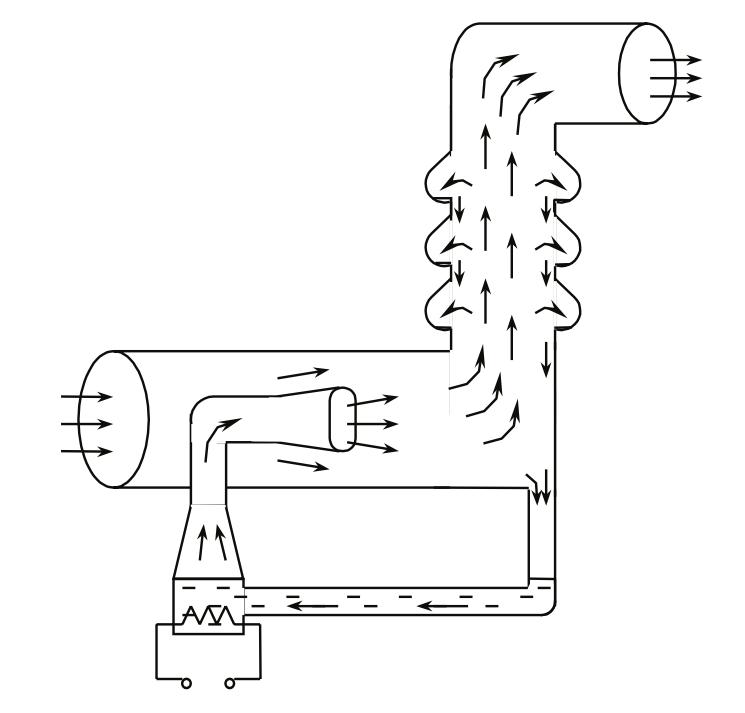
\includegraphics[scale=0.2]{3.jpg} 
	\caption{Схема работы одной ступени диффузионного насоса} 
\end{wrapfigure}


Устройство одной ступени масляного диффузионного насоса схематически показано на Рис. 3 (в лабораторной установке используется несколько откачивающих ступеней). Масло, налитое в сосуд, подогревается электрической печкой. Пары масла поднимаются по трубе и вырываются из сопла. Струя паров увлекает молекулы газа, которые поступают из откачиваемого сосуда через трубку. Дальше смесь попадает в вертикальную трубу. Здесь масло осаждается на стенках трубы и маслосборников и стекает вниз, а оставшийся газ откачивается форвакуумным насосом. 



\newpage

  
 \subsection*{Процесс откачки}
Опишем процесс откачки математически: 
Пусть W --- объем газа, удаляемого из сосуда при данном давлении за единицу времени, $Q_i$ для различных значений $i$ обозначим различные притоки газа в сосуд (в единицах $PV$), такие как течи извне $Q_\text{и}$, десорбция с поверхностей внутри сосуда $Q_\text{д}$, обратный ток через насос $Q_\text{н}$. Тогда, приравнивая убыль газа из сосуда (с точностью до $RT/\mu$) в единицу времени $-VdP$ и сумму перечисленных токов имеем:
 \begin{equation}
 	-VdP = (PW - \sum_i Q_i)dt
 \end{equation}
 При достижении предельного вакуума устанавливается давление $P_{\text{пр}}$, и $dP = 0$. Тогда
 \begin{equation}
 	 W = ( \sum_i Q_i )/P_{\text{пр}}
 \end{equation}
 Поскольку обычно $Q_\text{и}$ постоянно, а $Q_\text{н}$ и $Q_\text{д}$ слабо зависят от времени, также считая постоянной W, можем проинтегрировать (1) и получить:
 \begin{equation}
 	P - P_{\text{пр}} = (P_0 - P_{\text{пр}})\exp(-\frac{W}{V}t)
 \end{equation}
Полная скорость откачки $W$, собственная скорость откачки насоса $W_{\text{н}}$ и проводимости элементов системы $C_1, C_2,...$ соотносятся согласно формуле (4), и это учтено в конструкции установки.
 \begin{equation}
 \frac{1}{W} = \frac{1}{W} + \frac{1}{C_1} + \frac{1}{C_2} + ...
\end{equation}

\newpage

\subsection*{Течение газа через трубу}
Характер течения газа существенно зависит от соотношения между размерами системы и длиной свободного пробега молекул. При атмосферном и форвакуумном давлениях  длина свободного пробега меньше диаметра трубок, и течение газа определяется его вязкостью, т.е. взаимодействием молекул. При высоком вакууме течение существеннее определяется взаимодействием со стенками \\
Для количества газа, протекающего через трубу длины $l$ и радиуса $r$ в условиях высокого вакуума, справедлива формула:
\begin{equation}
	\frac{d(PV)}{dt} = \frac{4}{3}r^3\sqrt{\frac{2\pi RT}{\mu}}\frac{P_2 - P_1}{l}
\end{equation}
Если труба соединяет насос установку, то давлением $P_1$ у насоса можно пренебречь. Давление в сосуде $P = P_2$. Тогда имеем:
\begin{equation}
C_\text{тр} = \left(\frac{dV}{dt}\right)_\text{тр} = \frac{4r^3}{3l}\sqrt{\frac{2\pi RT}{\mu}}
\end{equation}

\section*{Ход работы}

\paragraph{Определение объёмов форвакуумной и высоковакуумной частей установки.}

\subparagraph{1.} Перед началом работы проверим, что все краны приведены в правильное положение. 

\subparagraph{2.} Запустим воздух в систему (для этого нужно открыть кран $К_2$  и подождать пару минут пока воздух заполнит установку). 

\subparagraph{3.} Запустим форвакуумный насос, чтобы он откачал воздух из установки. 

Пронаблюдаем за тем, как давление в установке уменьшается и продолжим откачку до момента, пока давление не будет порядка $ 10^{-2}~мм~рт.~ ст.$. Запишем итоговое значение: 

$
P_0 = (1.2 \pm 0.1) \cdot 10^{-2}~мм~рт.~ ст.
$

\subparagraph{4.} Отсоединим установку от форвауумного насоса, а затем объём, заключенный в кранах и капиллярах форвакуумной части, откроем на всю форвакуумную часть. Тогда давление изменится

\subparagraph{5.} Запишем показания маслянного манометра, а именно высоту масла в обоих коленах: 

$
h_1 = (34.5 \pm 0.1)~см~масл. ~ст.,\quad  h_2 = (5.7 \pm 0.1)~ см ~масл. ~ст.,
$

$\varepsilon_{\Delta h} = \sqrt{\varepsilon_{\Delta h1}^2 + \varepsilon_{\Delta h2}^2}\approx 2.5 \%$

$
\Delta h_{фв} = (28.8 \pm 0.7) ~ см ~масл. ~ст.
$

\subparagraph{6.} Зная объём "запертой"  части установки $V_{кап} = 50 ~ см^3$ (он указан на установке) и используя соотношение $P_1/P_2=V_2/V_1$ вычислим объём форвауумной части установки. При этом давление $P_1 = P_{атм} = (101.4 \pm 0.05) ~ кПа$ $P_2 = \Delta h_{фв}  \rho_{масл} g$, а относительная погрешность полученного значения равна относительной погрешности величины $\Delta h_{фв} $ 
$
\varepsilon_V = \varepsilon_{P_1} \approx 2.5\%
$
(пренебрегаем погрешностью измерения атмосферного давления $\varepsilon_{P_{атм}} \approx 0.05 \%$) и в результате имеем: 

$
V_{фв} = (1.96 \pm 0.06)~ л
$

\subparagraph{7.} Проведём те же самые измерения с диффузионным насосом и получим объём установки, из которой вычитанием объёма форвакуумной части получается объём высоковакуумной части. 

$
h_1 = (29.5 \pm 0.1)~см~масл. ~ст., \quad h_2 = (11.5\pm 0.1)~ см ~масл. ~ст.,
$


$
\Delta h_{вв} = (18 \pm 0.5) ~ см ~масл. ~ст.,
$

Погрешности высот определяются аналогично предыдущему пункту. 

$
\varepsilon_V = \varepsilon_{P_2}
$
(пренебрегаем погрешностью измерения атмосферного давления $\varepsilon_{P_{атм}} \approx 0.05 \%$)

$
V = V_0 \dfrac{P_1}{P_2} \approx (3.04 \pm 0.10) ~ л,
$

$
\sigma_{V_{вв}} = \sqrt{\sigma_{V_{фв}}^2 + \sigma_{V}^2} \approx 0.11~л,
$

 В результате искомая величина равна: 

$
V_{вв} = (1.08 \pm 0.11) ~ л.
$


\paragraph{Получение высокого вакуума и измерение скорости откачки.}

\subparagraph*{8.} Не выключая форвакуумного насоса убедимся в том, что в установке не осталось запертых объёмов. 

\subparagraph*{9.} Откачав установку до давления порядка $ 10^{-2}~мм~рт.~ ст.$, приступим к откачке ВБ с помощью диффузионного насоса. 


\subparagraph*{10.} С помощью термопарного манометра пронаблюдаем за тем, как идёт откачка ВБ. Мы должны продолжать процесс откачки до тех пор, пока там не установится давление порядка $3 \cdot 10^{-4}~мм~рт.~ ст.$ При приближении давления к этой величине масло в диффузионном насосе закипит, поэтому подсчитаем количество капель, стекающих из сопла второй ступенидиффузионного насоса: 

$
N = 16 ~ капель. 
$


\subparagraph*{11.} С помощью ионизационного манометра измерим значение предельного давления в системе со стороны высоковакуумной части: 

$
P_{пр} = (7.5 \pm 0.1)  \cdot 10^{-5} ~мм ~рт. ~ст.
$


\subparagraph*{12.} Найдём скорость откачки по ухудшению и улучшению вакуума, для этого открывая и закрывая кран $К_3$ будем то подключать насос к объёму, то отключать его, при этом на видео зафиксируем показания манометра от времени и занесём полученные результаты в Таблицу 1 и построим графики необоходимых  зависимостей (каких именно подробнее описано в соответствующх пунктах ниже), для которых определим коэффициенты наклона прямых и их погрешности (с помощью МНК), полученные результаты также зафиксируем в Таблице 1. Так же запишем итоговое значение для коэффициента наклона прямых, которое является средним из двух полученных, а его погрешность вычисляется по формуле $\sigma_k = \sqrt{\sigma_{k_1}^2 + \sigma_{k_2}^2}$ или же полуразность $k_1$ и  $k_2$, если вдруг эти значения не будут совпадать в пределах погрешности $k_1$ и $k_2$.



\begin{table}[h!]
	\centering 
	\caption{Результаты измерений}
	\begin{tabular}{|l|l|l|l|l|l|l|l|} \hline 
		\multicolumn{4}{|c|}{Улучшение} & \multicolumn{4}{|c|}{Ухудшение} \\ \hline
		$P, \cdot 10^{-5}~ торр$ & $t, с$ &$P, \cdot 10^{-5}~ торр$ & $t, с$ &$P, \cdot 10^{-5}~ торр$ & $t, с$ &$P, \cdot 10^{-5}~ торр$ & $t, с$  \\ \hline
		72 & 0 & 72 & 0 & 7.6 & 0 & 8.5  & 0 \\ \hline 
		68 & 1 & 69 & 1 & 10 & 7 & 14 & 7 \\ \hline 
		57 & 2 & 58 & 2 & 19 & 14 & 22 & 14 \\ \hline 
		43 & 3 & 40 & 3 & 26 & 21 & 28 & 21 \\ \hline 
		32 & 4 & 32 & 4 & 33 & 28 & 37 & 28 \\ \hline 
		24 & 5 & 25 & 5 & 35 & 35 & 44 & 35 \\ \hline
		19 & 6 & 21 & 6 & 38 & 42 & 51 & 42 \\ \hline 
		17 & 7 & 17 & 7 & 44 & 49 & 55 & 49 \\ \hline
		14 & 8 & 15 & 8 & 51 & 56 & 58 & 56 \\ \hline 
		12 & 9 & 14 & 9 & 58 & 63 & 65 & 63 \\ \hline
		11 & 10 & 12 & 10 & 65 & 70 & 72 & 70 \\ \hline 
		10 & 11 & 10 & 11 & 71 & 77 &    &    \\ \hline
		9.8 & 12 & 9.8 & 12 &    &    &      &       \\ \hline
		9.5 & 13 & 9.5 & 13 &    &    &      &       \\ \hline 
		9.3 & 14 & 9.1 & 14 &    &    &      &       \\ \hline 
		\multicolumn{4}{|l|}{$k_1 = -(0.298 \pm 0.002) ~  с^{-1}$} & \multicolumn{4}{|l|}{$k_1 = (0.812\pm 0.005) ~ \cdot 10^{-5} ~торр \cdot с^{-1}$} \\ 
		
		\multicolumn{4}{|l|}{$k_2 = -(0.285 \pm 0.003) ~ с^{-1}$}
		&\multicolumn{4}{|l|}{$k_2 = (0.830 \pm 0.005) ~ \cdot 10^{-5} ~торр \cdot с^{-1}$} \\ 
		
		
		\multicolumn{4}{|l|}{$k_{ср} = -(0.291 \pm 0.006) ~ с^{-1}$}
		&\multicolumn{4}{|l|}{$k_{ср} = (0.821 \pm 0.07) ~ \cdot 10^{-5} ~ торр \cdot с^{-1}$} \\ 
		\hline
		
		
		
	\end{tabular}
\end{table}




\newpage

\begin{figure} [h!]
	\caption{Улучшение вакуума 1}
	\centering 
	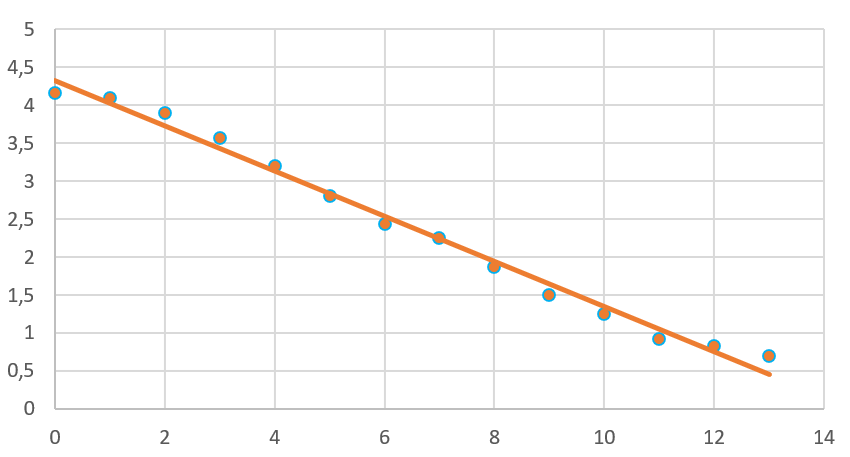
\includegraphics[scale=0.8]{Улучшение1.png} 
\end{figure}

\begin{figure} [h!]
	\caption{Улучшение вакуума 2}
	\centering 
	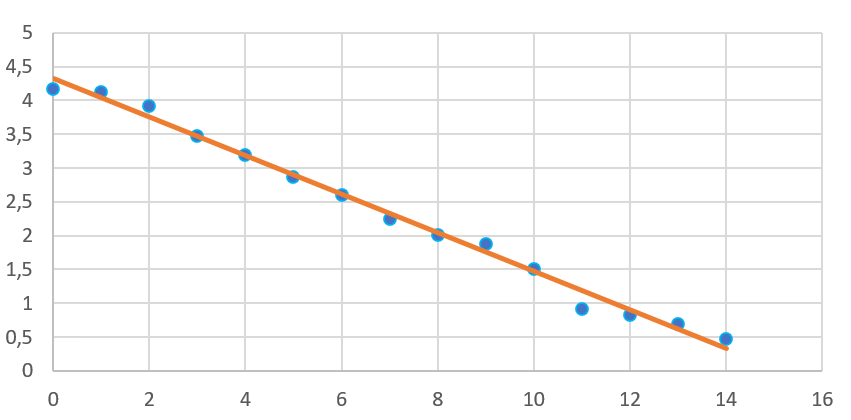
\includegraphics[scale=0.8]{Улучшение2.png} 
\end{figure}


\newpage

\begin{figure} [h!]
	\caption{Ухудшение  вакуума 1}
	\centering 
	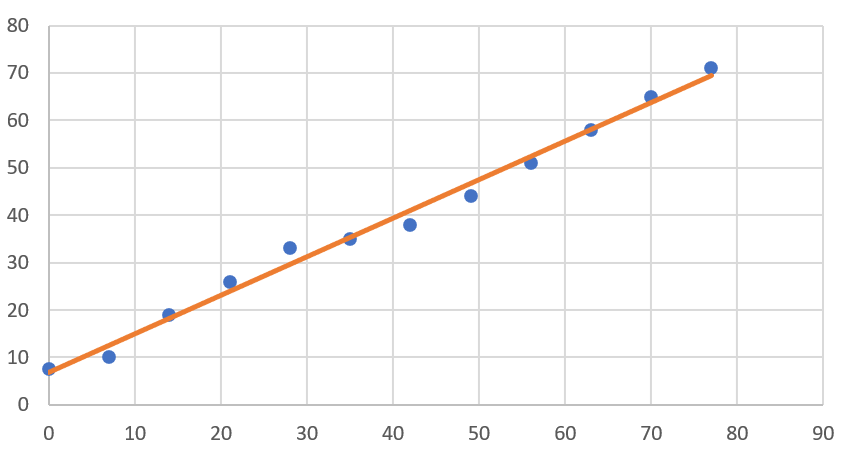
\includegraphics[scale=0.8]{Ухудшение1.png} 
\end{figure}

\begin{figure} [h!]
	\caption{Ухудшение  вакуума 2}
	\centering 
	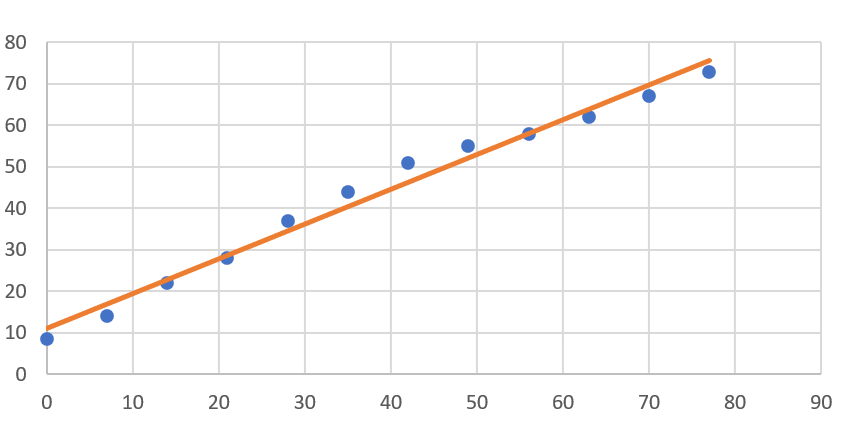
\includegraphics[scale=0.8]{Ухудшение2.png} 
\end{figure}

Сначала проведём вычисления для коэффициента $k$, полученного при улучшении вакуума (для этого мы строили графики зависимости $\ln (P-P_{пр})$ от $t$). Поскольку $W = -kV_{вв}$, то $\varepsilon_W = \sqrt{\varepsilon_k^2 + \varepsilon_{V_{вв}}^2} \approx 4\%$, в результате имеем: 

$
W = (0.31 \pm 0.01) ~ л /с.
$


\subparagraph*{13.} Оценим величину потока газа  $Q_Н$. Для этого воспользуемся данными, полученными при ухудшении вакуума. А именно построим графики зависимости $P(t)$ и определим для них коэффициенты угла наклона прямой. Поскольку $V_{вв}dP = (Q_Д + Q_И) dt$ получим $(Q_Д + Q_И) = kV_{вв} = (0.88 \pm 0.08)~ \cdot 10^{-5} ~торр \cdot л / c $ (Погрешность рассчитывается по формуле $\varepsilon =  \sqrt{\varepsilon_k^2 + \varepsilon_{V_{вв}}^2} \approx 10\%$). 


 Используя формулу $Q_Н = P_{пр}W - (Q_Д + Q_И)$, а значит $\varepsilon_{Q_Н} =  \sqrt{\varepsilon_{P_{пр}W}^2 + \varepsilon^2} \approx 11\%$ получим, что: 
 
 $
 Q_Н = (1.45 \pm 0.16) \cdot 10^{-5} ~ торр \cdot л / с.
 $
 
 

\subparagraph*{14.} Оценим пропускную способность трубки по формуле (6):

$
L = (10 \pm 1)~ см; \quad   d = (0.8 \pm 0.1) ~ мм.
$ 

$
C_{тр} = (1.0 \pm 0.2)\cdot 10^{-8} ~ торр \cdot л / с.
$
 
Погрешность $C_{тр}$  оценена как корень из суммы квадратов погрешностей длинны и диаметра (которые явням образом не указаны на установке, поэтому скорее всего оценка довольно грубая). 

\subparagraph*{15.} Введём в систему исскуственную течь и запишем значение  установившегося при этом давления и давления $P_{фв}$: 


$
P_{уст} = (1.3 \pm 0.1) \cdot 10^{-4} ~ торр.
$

$
P_{фв} = (2.5 \pm 0.1) \cdot 10^{-3} ~ торр.
$


\subparagraph*{16.} Поскольку

$$
P_{пр} W = Q_1, \quad P_{уст} W = Q_1 + \frac{d(PV)_{кап}}{dt}, 
$$

то 

$$
W = \frac{d(PV)_{кап}}{dt}\frac{P_{фв}}{P_{ уст}-P_{пр}} = (0.20 \pm 0.05) ~см^3 \cdot c;
$$


(Поскольку давления померены с точностью не менее $10\%$, то можно учитывать погрешность, вносимую величиной $\frac{d(PV)_{кап}}{dt}$ относительная погрешность которой равна относительной погрешности $C_{тр}$, то есть составляет $20\%$)


\subparagraph*{17.} Следуя указаниям в методичке выключаем установку. 


\section*{Вывод}

В ходе данной работы было проверено несколько методик по измерению производительности высоковакуумного насоса. Удалось проверить законы, в соответстви с которыми вакуум в установке ухудшается и улучшается, в хорошем результате помогают убедиться графики, на которых прослеживается достаточно чёткая линейная зависимость (для улучшения вакуума -- линейная зависимость $\ln (P-P_{пр})$ от $t$, а для ухудшения -- $P(t))$.  





\end{document}